\section{Durchführung}
\label{sec:Durchführung}

Für den Versuchsaufbau wird eine $\SI{100}{\centi\meter}$ lange Führungsschiene verwendet, auf der alle Mess- und Versuchsinstrumente befestigt werden.
Dabei wird versucht, den Abstand zwischen Spalt und Lichtstärkesensor so groß wie möglich zu halten.
Ein He-Ne-Laser mit einer Wellenlänge von $\lambda = \SI{633}{\nano\meter}$ wird als kohärente Lichtquelle verwendet.

\begin{figure}
    \centering
    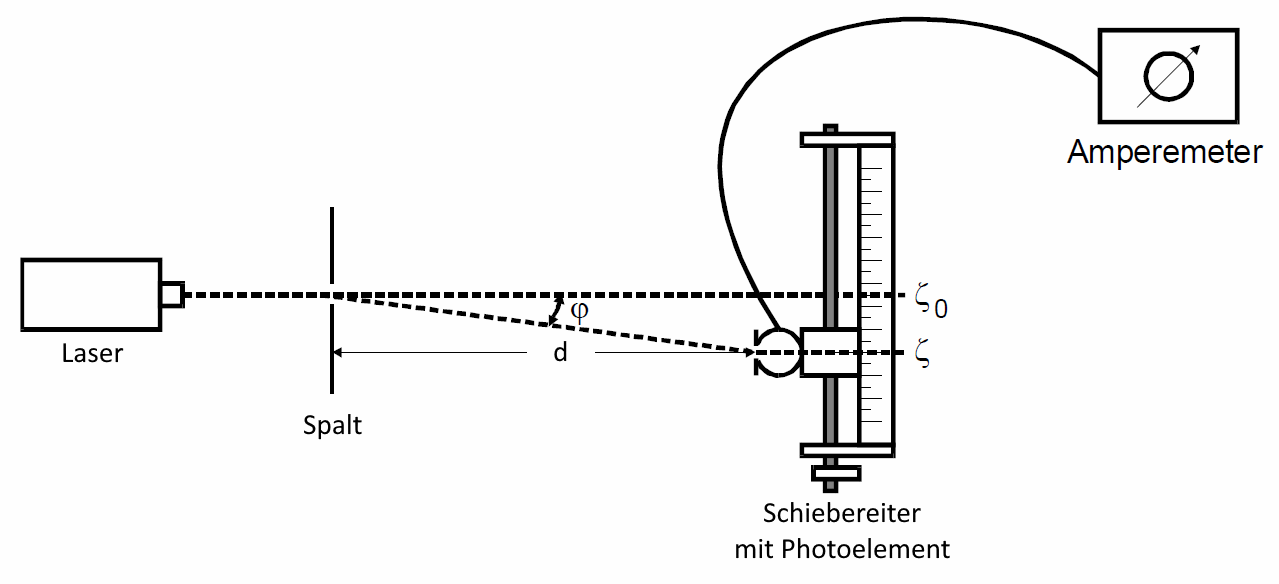
\includegraphics[width=\textwidth]{plots/Versuchsaufbau.png}
    \caption{Schematischer Versuchsaufbau.\protect\footnotemark}
    \label{fig:schemAufbau}
\end{figure}

\FloatBarrier

Die Instrumente müssen kalibriert und der Laser vorgeheizt werden.
Zur Kalibrierung wird der Laser und die Spaltblende derart ausgerichtet, dass der Lichtstrahl mittig auf den zu messenden Einzel- beziehungsweise Doppelspalt trifft.
Für die Messungen des Beugungsmusters wird ein Photosensor verwendet, welcher einen schmalen Spalt als Öffnung besitzt, der in Richtung des Lasers ausgerichtet wird.
Der Photosensor wird mit einem Amperemeter ausgelesen und misst die Lichtintensität. Für eine genaue Auswertung der Daten muss der Dunkelstrom $I_d$ bestimmt werden.
$I_d$ ist die Stromstärke, die der Photosensor im Leerlauf misst; also bei fertigem Aufbau, aber ausgeschaltetem Laser.\\
Das Beugungsbild muss bei eingeschaltetem Laser vertikal mittig auf das Photoelement treffen.
Die Kalibrierung ist abgeschlossen, wenn sichergestellt ist, dass sich Laser und Spalthalterung nicht mehr bewegen können und das Photoelement auf dem Schieberegler hinreichend nach links
und rechts verstellt werden kann.\\
\footnotetext{Zeichnung angelehnt an Versuchsanleitung.\cite{Versuchsanleitung}}

\begin{figure}
    \centering
    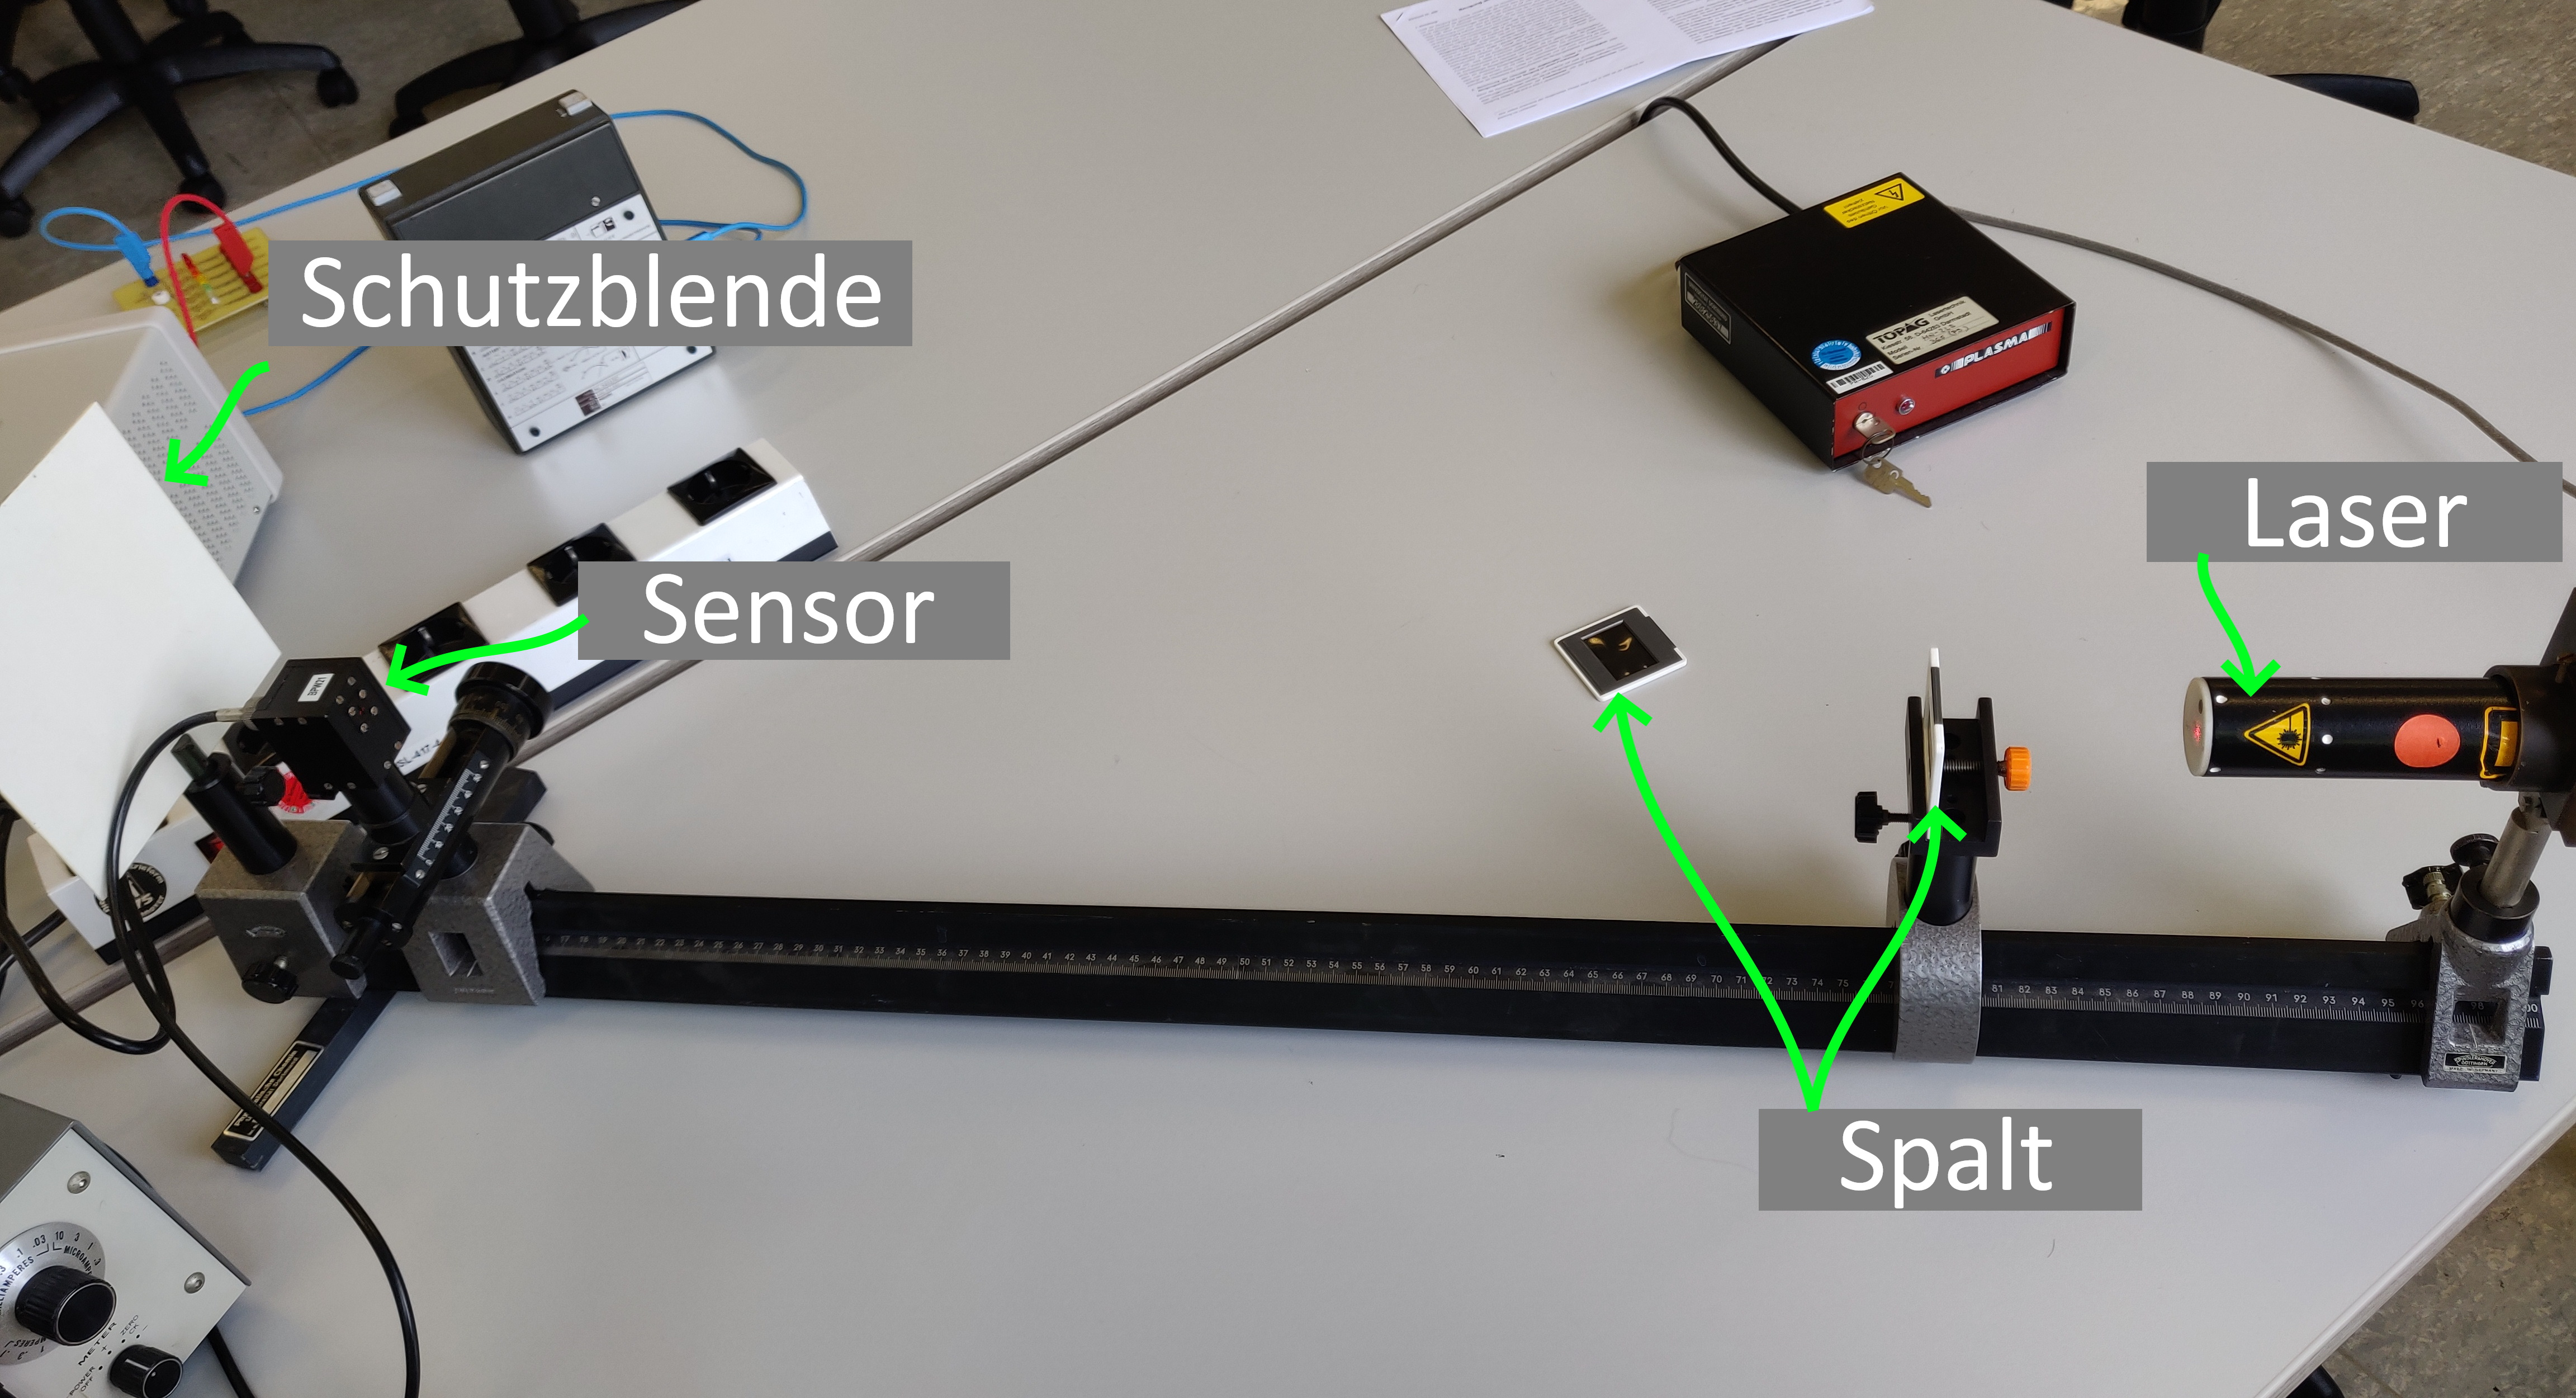
\includegraphics[width=\textwidth]{plots/tatVersuchsaufbau.jpg}
    \caption{Realer Versuchsaufbau.}
    \label{fig:tatVersuchsaufbau}
\end{figure}

Es werden je nach Verfügbarkeit der Blenden ein Einzel- und ein Doppelspalt gemessen.
Für die einzelnen Messungen wird der Sensor auf dem Schieberegler in äquidistanten Schritten von links nach rechts bewegt und die absoluten Abstände aufgeschrieben.
Jede Messreihe besteht aus mindestens 50 Messwerten.